\documentclass[ngerman]{dtk}
\ifluatex\else
  \usepackage[utf8]{inputenc}
\fi

\let\File\texttt
\let\Package\texttt

\begin{document}
\title{\enquote{Making \TeX\ Great Again} - Die TUG 2019 Tagung in Palo Alto}
\Author{Uwe}{Ziegenhagen}{Köln}
\maketitle

\begin{abstract}
Die TUG-Tagung zum 40.~Jubiläum von \TeX\ in Palo Alto gab mir Gelegenheit, in den Flieger zu steigen und die lange Reise nach Kalifornien anzutreten. Im folgenden Artikel möchte ich meine Eindrücke dieser Reise schildern und auf einige dort gehaltene Vorträge eingehen.
\end{abstract}

\section{Anreise}

Die Anreise nach Kalifornien begann morgens früh um 6:00 Uhr mit der Fahrt zum Kölner Hauptbahnhof. Köln ist glücklicherweise nur eine knappe ICE-Stunde vom Frankfurter Flughafen entfernt, der ICE war auch -- entgegen den Erfahrungen, die ich leider zu oft mit der Bahn machen darf -- pünktlich. Nicht pünktlich hingegen war die A380 der Lufthansa, die mich über den großen Teich bringen sollte:  nachdem alle Passagiere und das Gepäck eingeladen waren, kam die Meldung vom Kapitän, dass sich der Flug aufgrund technischer Probleme an einem Instrument auf unbestimmte Zeit verzögern würde. 

Glücklicherweise beherbergt der Frankfurter Flughafen nicht nur eine Menge Flugzeuge, sondern auch die entsprechenden Techniker,  daher konnten wir nach den Flug mit ungefähr zwei Stunden Verzögerung antreten, am Ende  sollte  sich die Zeit an Bord auf rund 14 Stunden summieren. 

Gepeinigt vom Jetlag -- die Zeitverschiebung zu Deutschland betrug neun Stunden -- kam ich Donnerstagmittag in San Francisco an. Da der vom Hotel in Palo Alto geforderte Preis für eine weitere Übernachtung völlig indiskutabel war, hatte ich vorab die Gelegenheit genutzt, mir über AirBnB ein Zimmer in San Francisco zu buchen. Müde, aber glücklich darüber, angekommen zu sein, fiel ich in einen tiefen Schlaf.

\section{Von San Francisco nach Palo Alto}

Am nächsten Tag schließlich ging es mit dem Zug knappe 50 Kilometer Richtung Süden nach Palo Alto, dem eigentlichen Tagungsort. Mit dem CalTrain gibt es eine Bahn-Verbindung, die von San Francisco aus über Menlo Park, Palo Alto, Mountain View in den Süden führt und dabei von den Pendlern genutzt wird, die sich kein Auto leisten können oder wollen. Die CalTrains sind doppelstöckige Züge, die aber für zwei Stockwerke eigentlich zu flach sind. Daher findet man im oberen Stockwerk keinen einzelnen durchgehenden Gang, sondern nur zwei recht schmale Stege sowie Einzelsitze. Im Vergleich dazu bieten moderne DB-Züge deutlich mehr Komfort.

Der geneigte Leser hat er sicher bereits an den Ortsnamen erkannt: Palo Alto liegt im Herzen des \enquote{Silicon Valley}, das seinen Wohlstand dem Silizium verdankt, das hier seit Jahrzehnten in Chip-Form gepresst wird. Seinen Aufstieg zu einem der wichtigsten Technologiestandorten begann 1951, als der Dekan der Stanford-Universität freie Landflächen der Universität für die Gründung des \enquote{Stanford Industrial Parks} nutzte und seine Studenten ermutigte, eigene Firmen zu gründen. Die Liste der Firmen, die dort ihren Sitz hatten und teilweise sogar heute noch haben, ist beeindruckend: Hewlett-Packard, IBM, Kodak, Apple, Intel, Cisco, Adobe, etc.

Palo Alto selbst hat knapp 70\,000 Einwohner und wurde nach \enquote{El Palo Alto}, einem besonders hohen Küstenmammutbaum (Sequoia sempervirens) benannt. Die Stadt wird zu großen Teilen von recht niedriger Bebauung geprägt, es gibt eine Vielzahl von sehr schönen Einfamilienhäusern, die verschiedenen Baustilen nachempfunden sind. Leider wirkt sich der Wohlstand des Silicon Valley gnadenlos auf die Preise aus.

Bei Quadratmeterpreisen von 20\,000 Euro, also ungefähr dem Doppelten dessen, was man in München für Eigentum bezahlt, müssen die Gehälter auch -- zumindest nach deutschem Maßstab -- astronomisch sein, wenn man nicht Fahrzeiten von mehreren Stunden täglich auf sich nehmen möchte oder kann.  

Doch nicht nur die Wohnkosten, auch die Lebenshaltungskosten gehören vermutlich in das obere Dezil der Lebenshaltungskosten in den USA. Ich habe noch nie so viele Tesla e-Autos gesehen wie dort, auch die Preise im Supermarkt schienen im Mittel das doppelte oder dreifache dessen zu betragen, was ich von deutschen Discountern gewohnt war.

Das intellektuelle Zentrum Palo Altos bildet natürlich die Stanford-Universität, die zu den besten Universitäten des Landes gehört. Aktuell lehren dort 21 Nobelpreisträger und vier Pulitzer-Preisträger, keine andere Universität hat mehr Turing Award Preisträger -- unter ihnen Donald Knuth -- hervorgebracht als Stanford. Der Campus besticht durch seine Größe und den exzellenten Zustand, bei einem kurzen Besuch vor meiner Rückreise konnte ich deutlich erkennen, was man mit den rund sechs Milliarden (!) US-Dollar pro Jahr, die Stanford als Budget hat, erreichen kann.

\section{Tag 0}

Am Donnerstagabend begann die TUG-Konferenz mit dem Willkommens-Empfang, eine gute Gelegenheit, um alte Kontakte zu treffen und neue Kontakte zu knüpfen. Ich war auch nicht der einzige Deutsche, mit Erik Braun vom CTAN-Team, Frank Mittelbach vom \LaTeX 3-Projekt, Martin Ruckert, dem Autor der MMIX-Ergänzung des Knuth-Opus \enquote{The Art of Computer Programming} und Henri Menke, dem PGF-Entwickler, hatten sich noch weitere Landsleute auf den Weg nach Palo Alto gemacht. Insgesamt war die TUG~2019 mit ca. 70 \TeX ies recht gut besucht, was sicherlich auch daran lag, dass Donald Knuth selbst sein Erscheinen angekündigt hatte.

\section{Tag 1}

Am Freitagmorgen wurde die Tagung offiziell durch den TUG-Präsidenten Boris Veytsman eröffnet, im Anschluss sprach Erik Braun über die technischen und organisatorischen Details von CTAN. Ihm folgte dann Arthur Reutenauer, der über die weitere Entwicklung von xe\TeX\ sprach. Auf Arthur folgten zwei Vorträge von Frank Mittelbach, die sich mit der Weiterentwicklung von \LaTeX 3 und der Behandlung von UTF8 in \LaTeX\ beschäftigten.

Frank ruft zwar auch interessierte \LaTeX-Nutzerinnen und Nutzer, jedoch insbesondere die Entwicklerinnen und Entwickler von \LaTeX-Paketen auf, die eigenen Pakete mit der aktuellen \LaTeX3-Version zu testen.



Nach der obligatorischen Kaffeepause hielt ich dann meinen ersten Vortrag mit dem Thema \enquote{Python und \LaTeX\ im Team}, den ich in ähnlicher Form bereits auf einer Dante-Tagung gehalten hatte.

Den folgenden Vortrag von Henri Menke fand ich ebenfalls sehr interessant. Er zeigte, wie man mittels LPEG-Parserbibliothek komplexe Datenstrukturen in Lua\LaTeX\ vearbeiten kann. 

Nach der Mittagspause gab es dann einen Vortrag von Richard Koch, dem \TeX shop Entwickler. Er sprach über die Sicherheitsanforderungen, die Apple an MacOS-Anwendungen stellt, und die Konsequenzen, die dies für ihn und anderen Mac\TeX\ Entwickler hat.

Der nächste Sprecher, Nate Stemen, kam von Overleaf, dem Anbieter des führenden Online-\TeX-Systems. Er sprach über die technische Infrastruktur, Nutzerzahlen und die Funktionen der Online-Lösung. Dem geneigten Leser sei empfohlen, sich diese Plattform einmal anschauen, sofern noch nicht geschehen. Sie nimmt ein großes Stück der Einstiegshürde, die vor der Nutzung von \TeX/\LaTeX steht, auch einige meiner Studentinnen und Studenten machen damit ihre ersten \TeX nischen Schritte.

Rishi T aus Indien war der nächste Sprecher, der \enquote{Neptune}, ein Proofing-Framework für \LaTeX-Autoren vorstellte. 

\begin{figure}
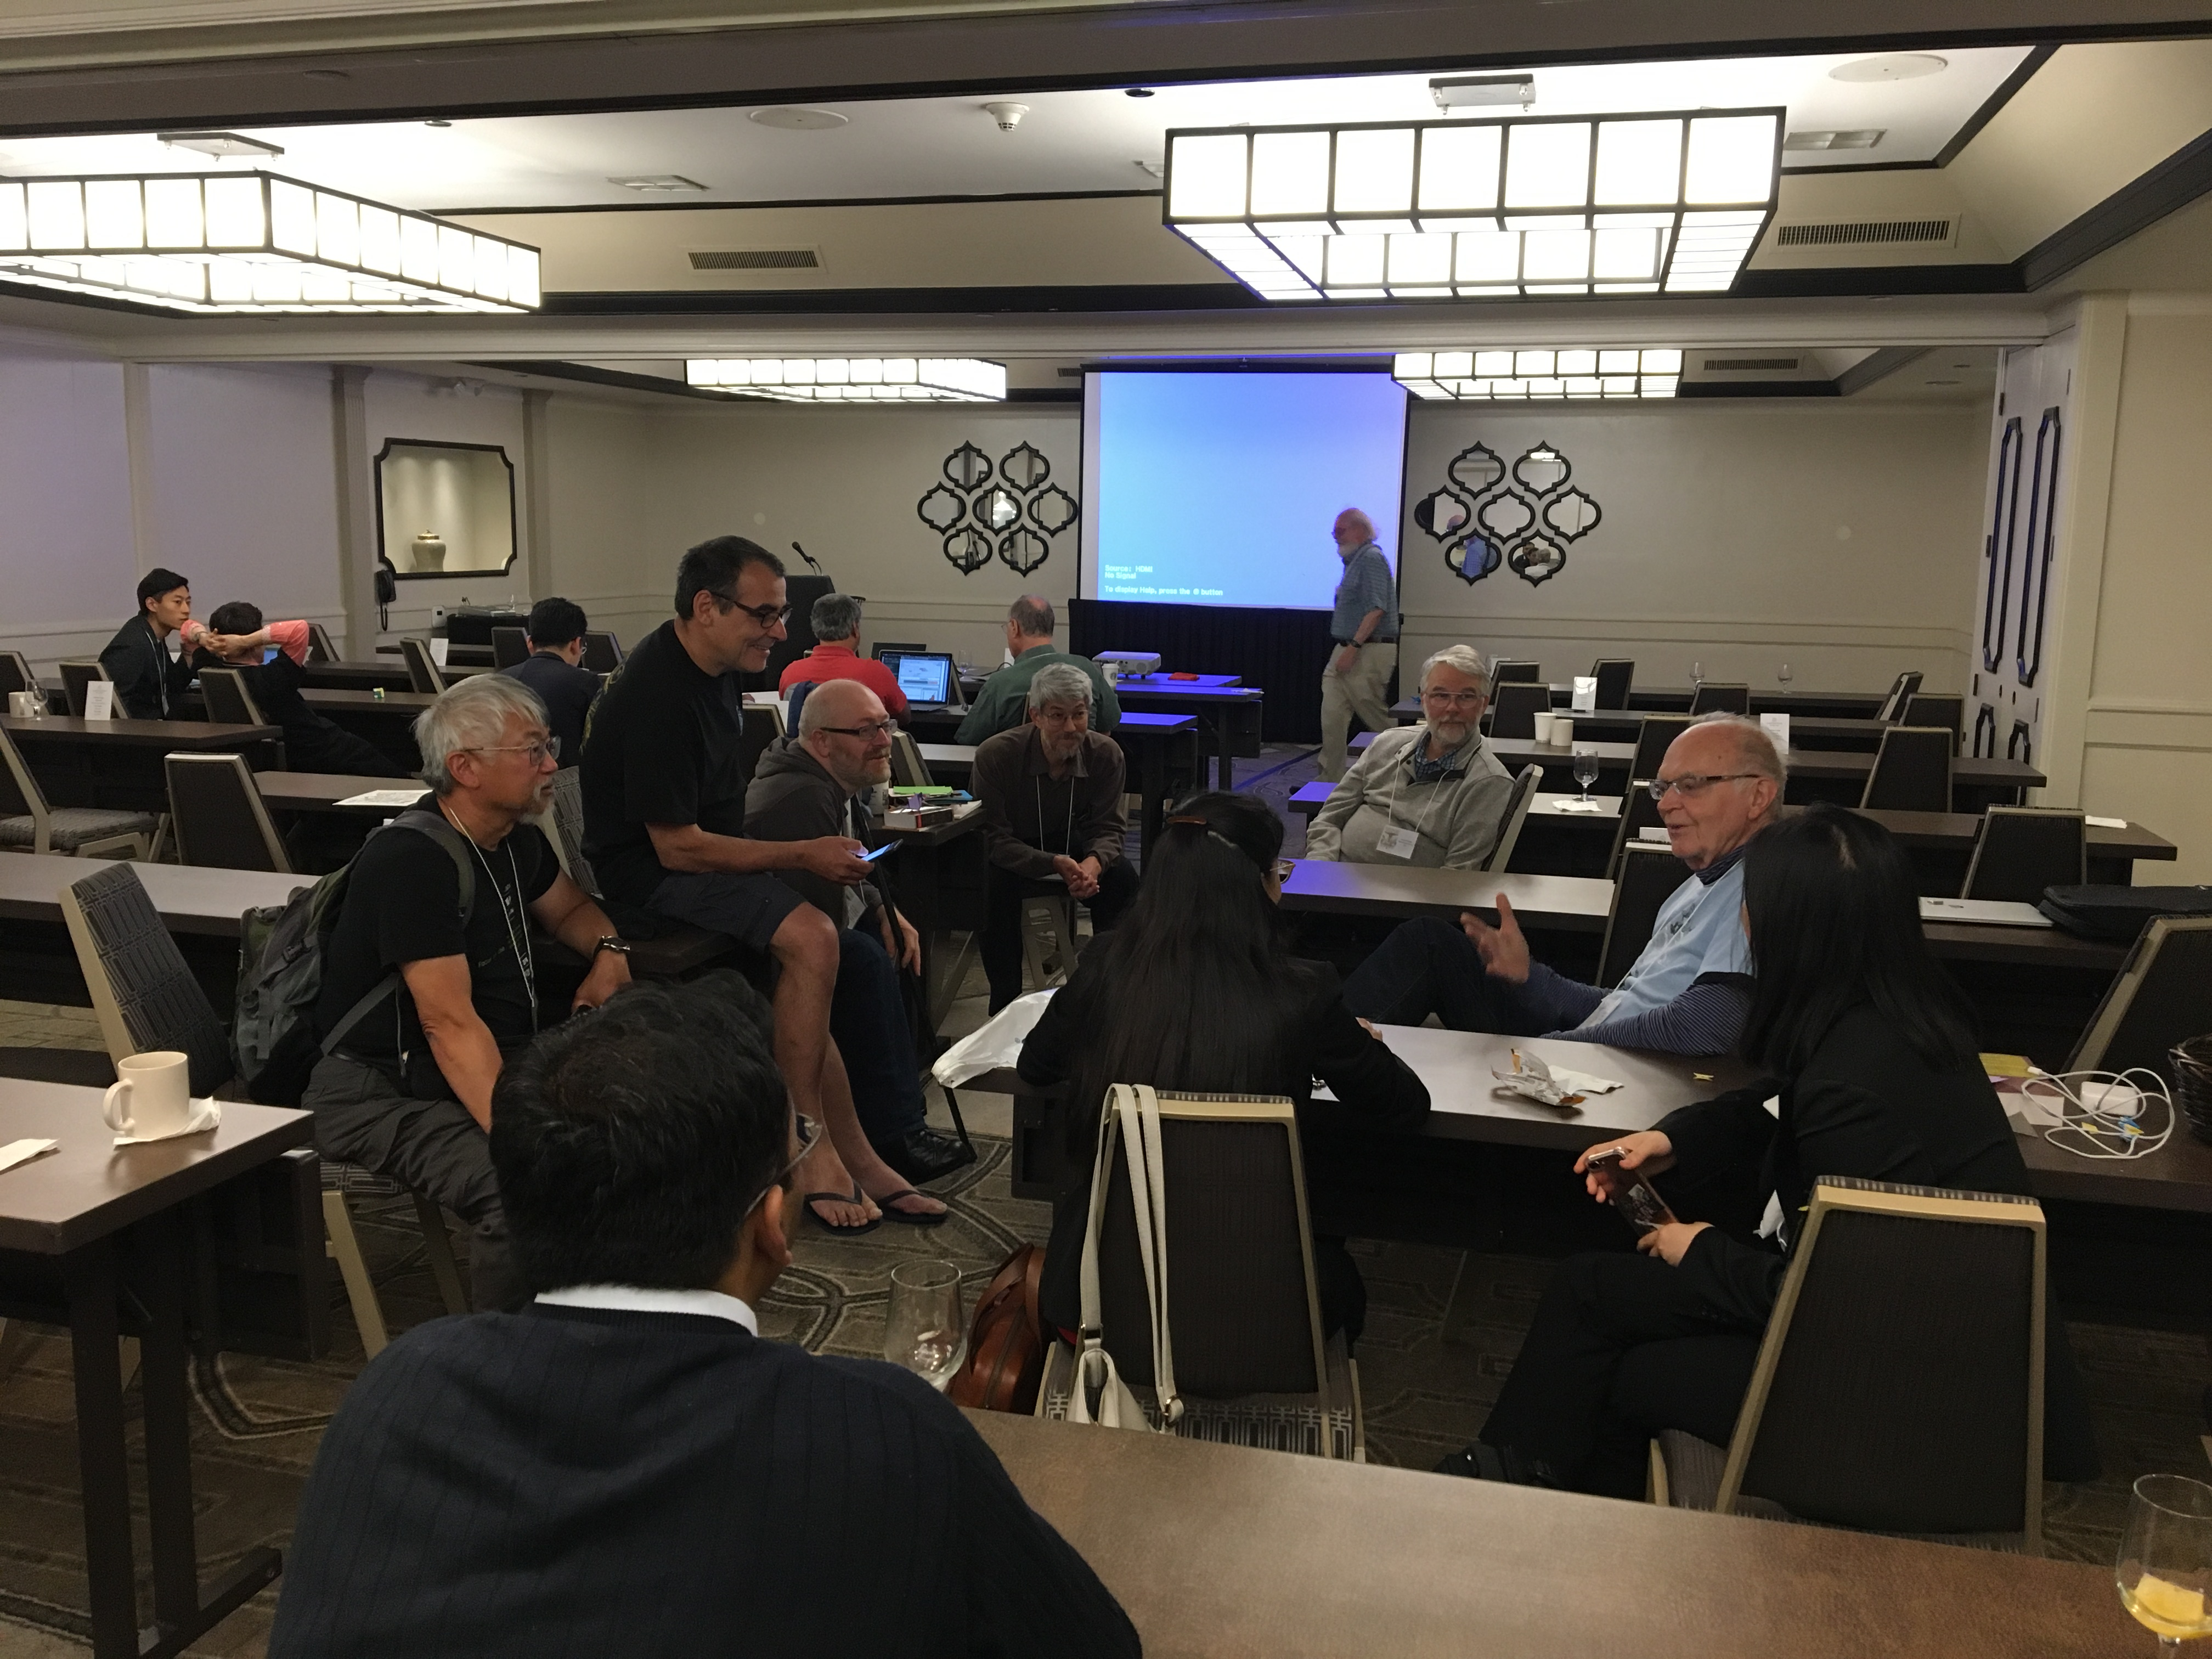
\includegraphics[width=\textwidth]{Juenger}
\caption{Donald Knuth, umgeben von einigen seiner \enquote{Jünger}}
\end{figure}

Der anschließende Vortrag Pavneet Aroras mit dem Titel \enquote{Rain Rain Go Away: Some thoughts on rain protection, and its uses } drehte sich vermutlich nur am Rande um \TeX/\LaTeX, ich persönlich konnte nur den Hinweis auf \enquote{Taskwarrior} mitnehmen, einer leichtgewichtigen Aufgabenverwaltung für unixoide Betriebssysteme.

\TeX-lastiger war dann der anschließende Vortrag von Shreevatsa R. Er beschrieb die Hindernisse, die man als Programmierer hat, wenn man denn den \TeX-Quellcode lesen und verstehen möchte und die Wege, diese Hindernisse zu überwinden.

Petr Sojka von CSTUG sprach anschließend über die große Verbreitung von \TeX, \LaTeX\ und Co in Tschechien, gefolgt von Shakthi Kannan, der eine Buchvorlage für xe\TeX\ vorstellte. Den Abschluss des Vortragsprogramms bildete dann Jim Hefferon, der darüber sprach, was heutige \TeX-Einsteiger erwarten würden.

\section{Tag 2}

Samstag, der zweite Tagungstag, begann mit einem Vortrag von Petr  und Ondřej Sojka, die über ihre Erfahrungen bei der Erstellung von tschechischen Trennmustern berichteten. Mit Trennmustern beschäftigte sich auch der folgende Vortrag von Arthur Reutenauer. Er sprach über die historische Entwicklung der Trennmuster-Verarbeitung in \TeX\ Live. Besonders interessant fand ich die Tatsache, das \TeX s Trennmusterlogik ihren Weg auch in \enquote{Konkurrenzprodukte} wie OpenOffice und LibreOffice gefunden hat.

Nach ihm präsentierte David Fuchs, \TeX-Pionier der ersten Stunde\footnote{\url{https://de.overleaf.com/blog/618-an-interview-with-david-fuchs-tex-pioneer-and-designer-of-the-dvi-file-format}} und Schöpfer des wohl den meisten vertrauten DVI-Formats. Er sprach darüber, was die Entwicklung der Rechenleistung in den letzten 40 Jahren möglich gemacht hat und zeigte ein -- wohl auf Metafont aufsetzendes -- System, das auf WYSIWYG-Art \TeX-Dokumente setzte. Es ist schade, dass die Vorträge dieser TUG-Tagung nicht auf Video aufgenommen wurden, diesen Vortrag hätte ich jedem empfohlen!

Tom Rokicki, bekannt als Entwickler von \texttt{dvips}, zeigte danach, wie man durchsuchbare PDFs mit Typ~3 Bitmapfonts erstellt. 

\begin{figure}[t]
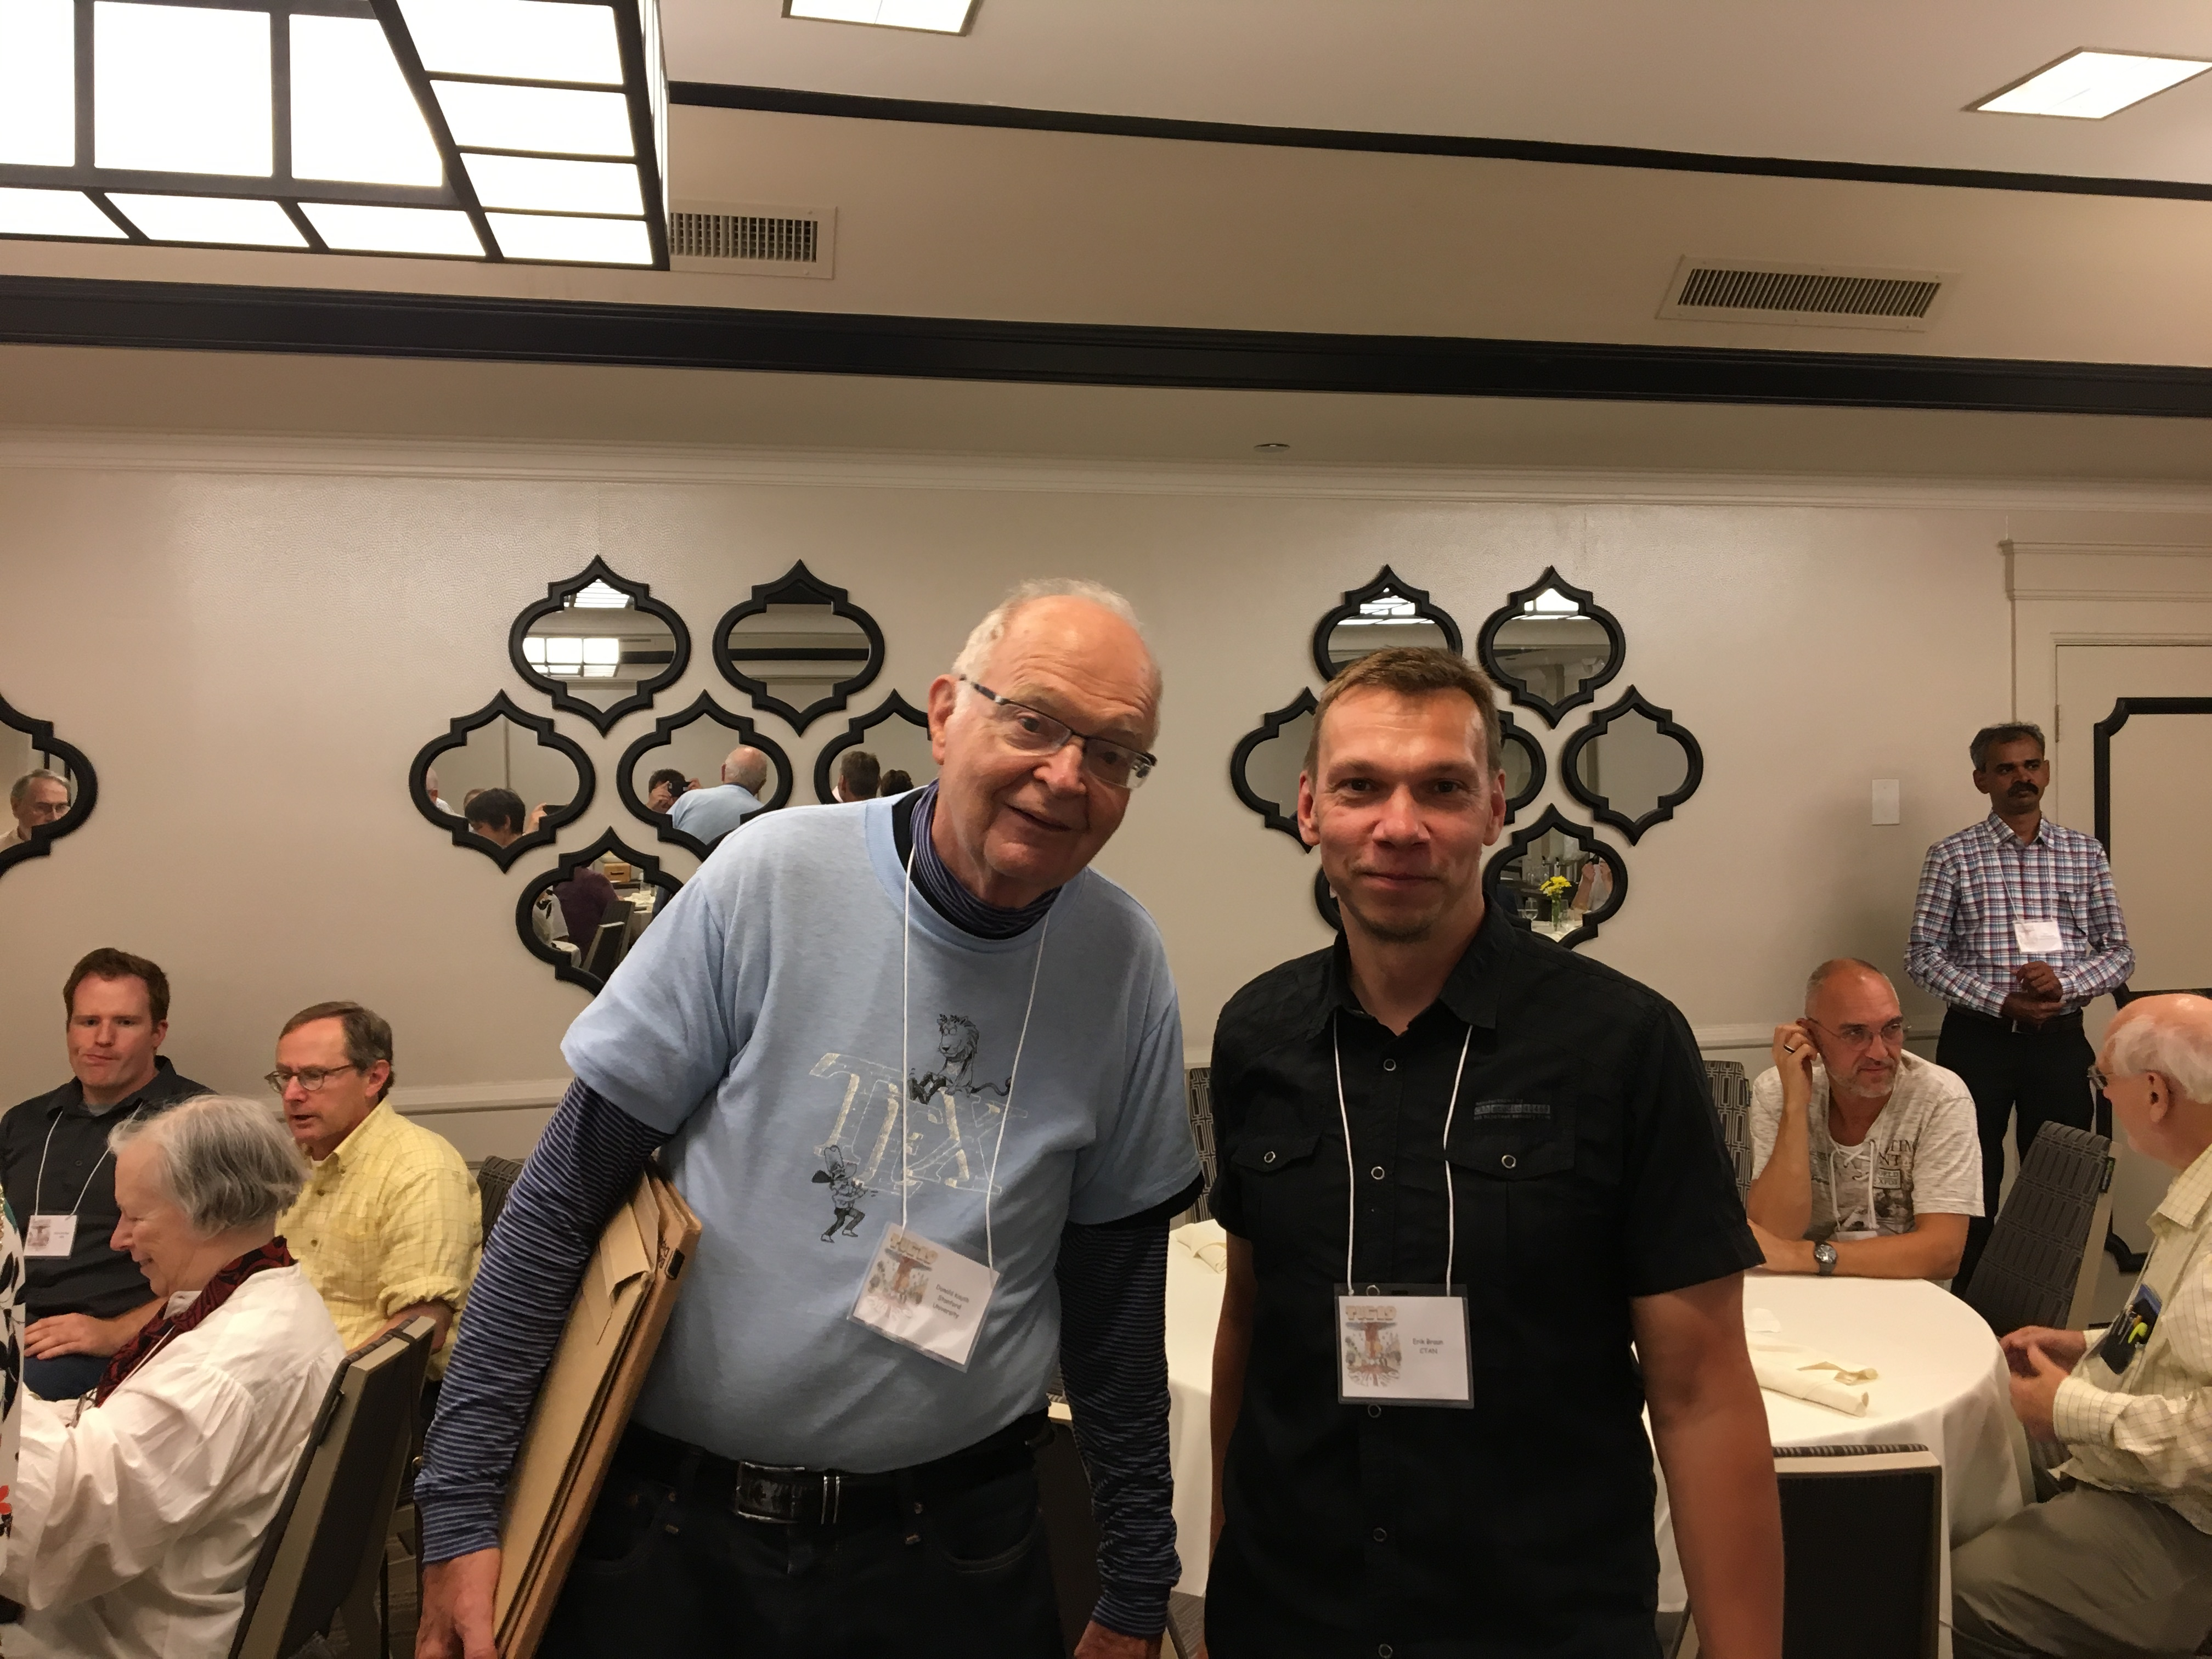
\includegraphics[width=\textwidth]{Don_Erik}
\caption{Donald Knuth und Erik Braun vom CTAN-Team}
\end{figure}


Vor der Mittagspause gab es dann noch einen tollen Vortrag von Douglas McKenna, der 
eine interaktive App über Hilbert-Kurven vorstellte. Die Besonderheit an dieser App ist, dass im Hintergrund ein speziell angepasster \TeX-Interpreter läuft. Die App ist für 8,99 Euro im Apple Appstore erhältlich und selbst dann sehr empfehlenswert, wenn man wenig mit Hilbert-Kurven zu tun hat.

Nach der Mittagspause sprach Jennifer Claudio dann über Kalligrafie im Textsatz bevor Federico Garcia über den perfekten Satz von Bindebögen im Notensatz sprach. Mit Unterbrechungen arbeitete er seit 2004 daran, den perfekten Bindebogen vorzustellen.

Vor der nachmittäglichen Kaffeepause sprach dann noch William Adams über ein System zur parametrischen Modellierung von verschiedenen 3D-Objekten, die dann auf CNC-Maschinen gefertigt werden. \LaTeX\ spielte dabei insofern eine Rolle, als dass die Parameter der Objekte in einem Lua\LaTeX\ Skript verarbeitet wurden,  das dann Schnittlisten und Bauanleitungen produzierte. Die Kickstarter-URL lautet \url{https://www.kickstarter.com/projects/designinto3d///design-into-3d-a-book-of-customizable-project-desi}

Nach der Pause am Nachmittag sprach dann der TUG-Präsident Boris Veytsman über die Erstellung kommentierter Editionen und ein neues \LaTeX-Paket, \enquote{commedit}, das er für die Erstellung dieser kommentierten Editionen geschrieben hat. Der interessierte Leser findet es unter \url{https://www.ctan.org/pkg/commedit}.

Die nächsten beiden Vorträge von Behrooz Parhami und Amine Anane behandelten dann den Satz von arabischen und persischen Schriften, bevor Takuto Asakura aus Japan über die synthetische Analyse von mathematischen Ausdrücken und natürlicher Sprache doziert.

\section{Tag~3}

Der dritte Tag der Konferenz begann mit einem Vortrag von Antoine Bossard zur Verbesserung des CJK-Supports in \XeTeX\ und Lua\TeX, gefolgt von einem Vortrag mehrerer Autoren zum Thema FreeType. Vor der Frühstückspause hielten Jennifer Claudio und Emily Park dann noch einen Vortrag zur Verbesserung von Koreanisch-Übersetzungen ins Englische.

Rishi T stellte im Anschluss daran mit \enquote{\TeX\ Folio} ein web-basiertes Publishing System vor, mit dem man aus XML-Inhalten verschiedene Output-Formate wie PDF und HTML erzeugen kann, gefolgt von einem Vortrag Boris Veytsmans zur Erzeugung von Bib\TeX\-Trainingsdaten. Ziel des Projekts ist die Nutzung von Machine Learning zum automatischen Parsen von Bibliographien, um so Verbindungen zwischen wissenschaftlichen Artikeln zu schaffen. Das Projekt nutzt dazu Nelson Beebes Archiv mit 1,4 Millionen (!) BibTeX-Einträgen, setzt diese mit 275 Bibliographie-Stilen aus dem aktuellen \TeX~Live und wendet dann die ML-Algorithmen auf das Ergebnis von 185 Millionen Literatur-Einträgen an. Nach Boris' Angaben wurden die Erkennungsergebnisse um den Faktor 5 verbessert.

\begin{figure}
\begin{center}
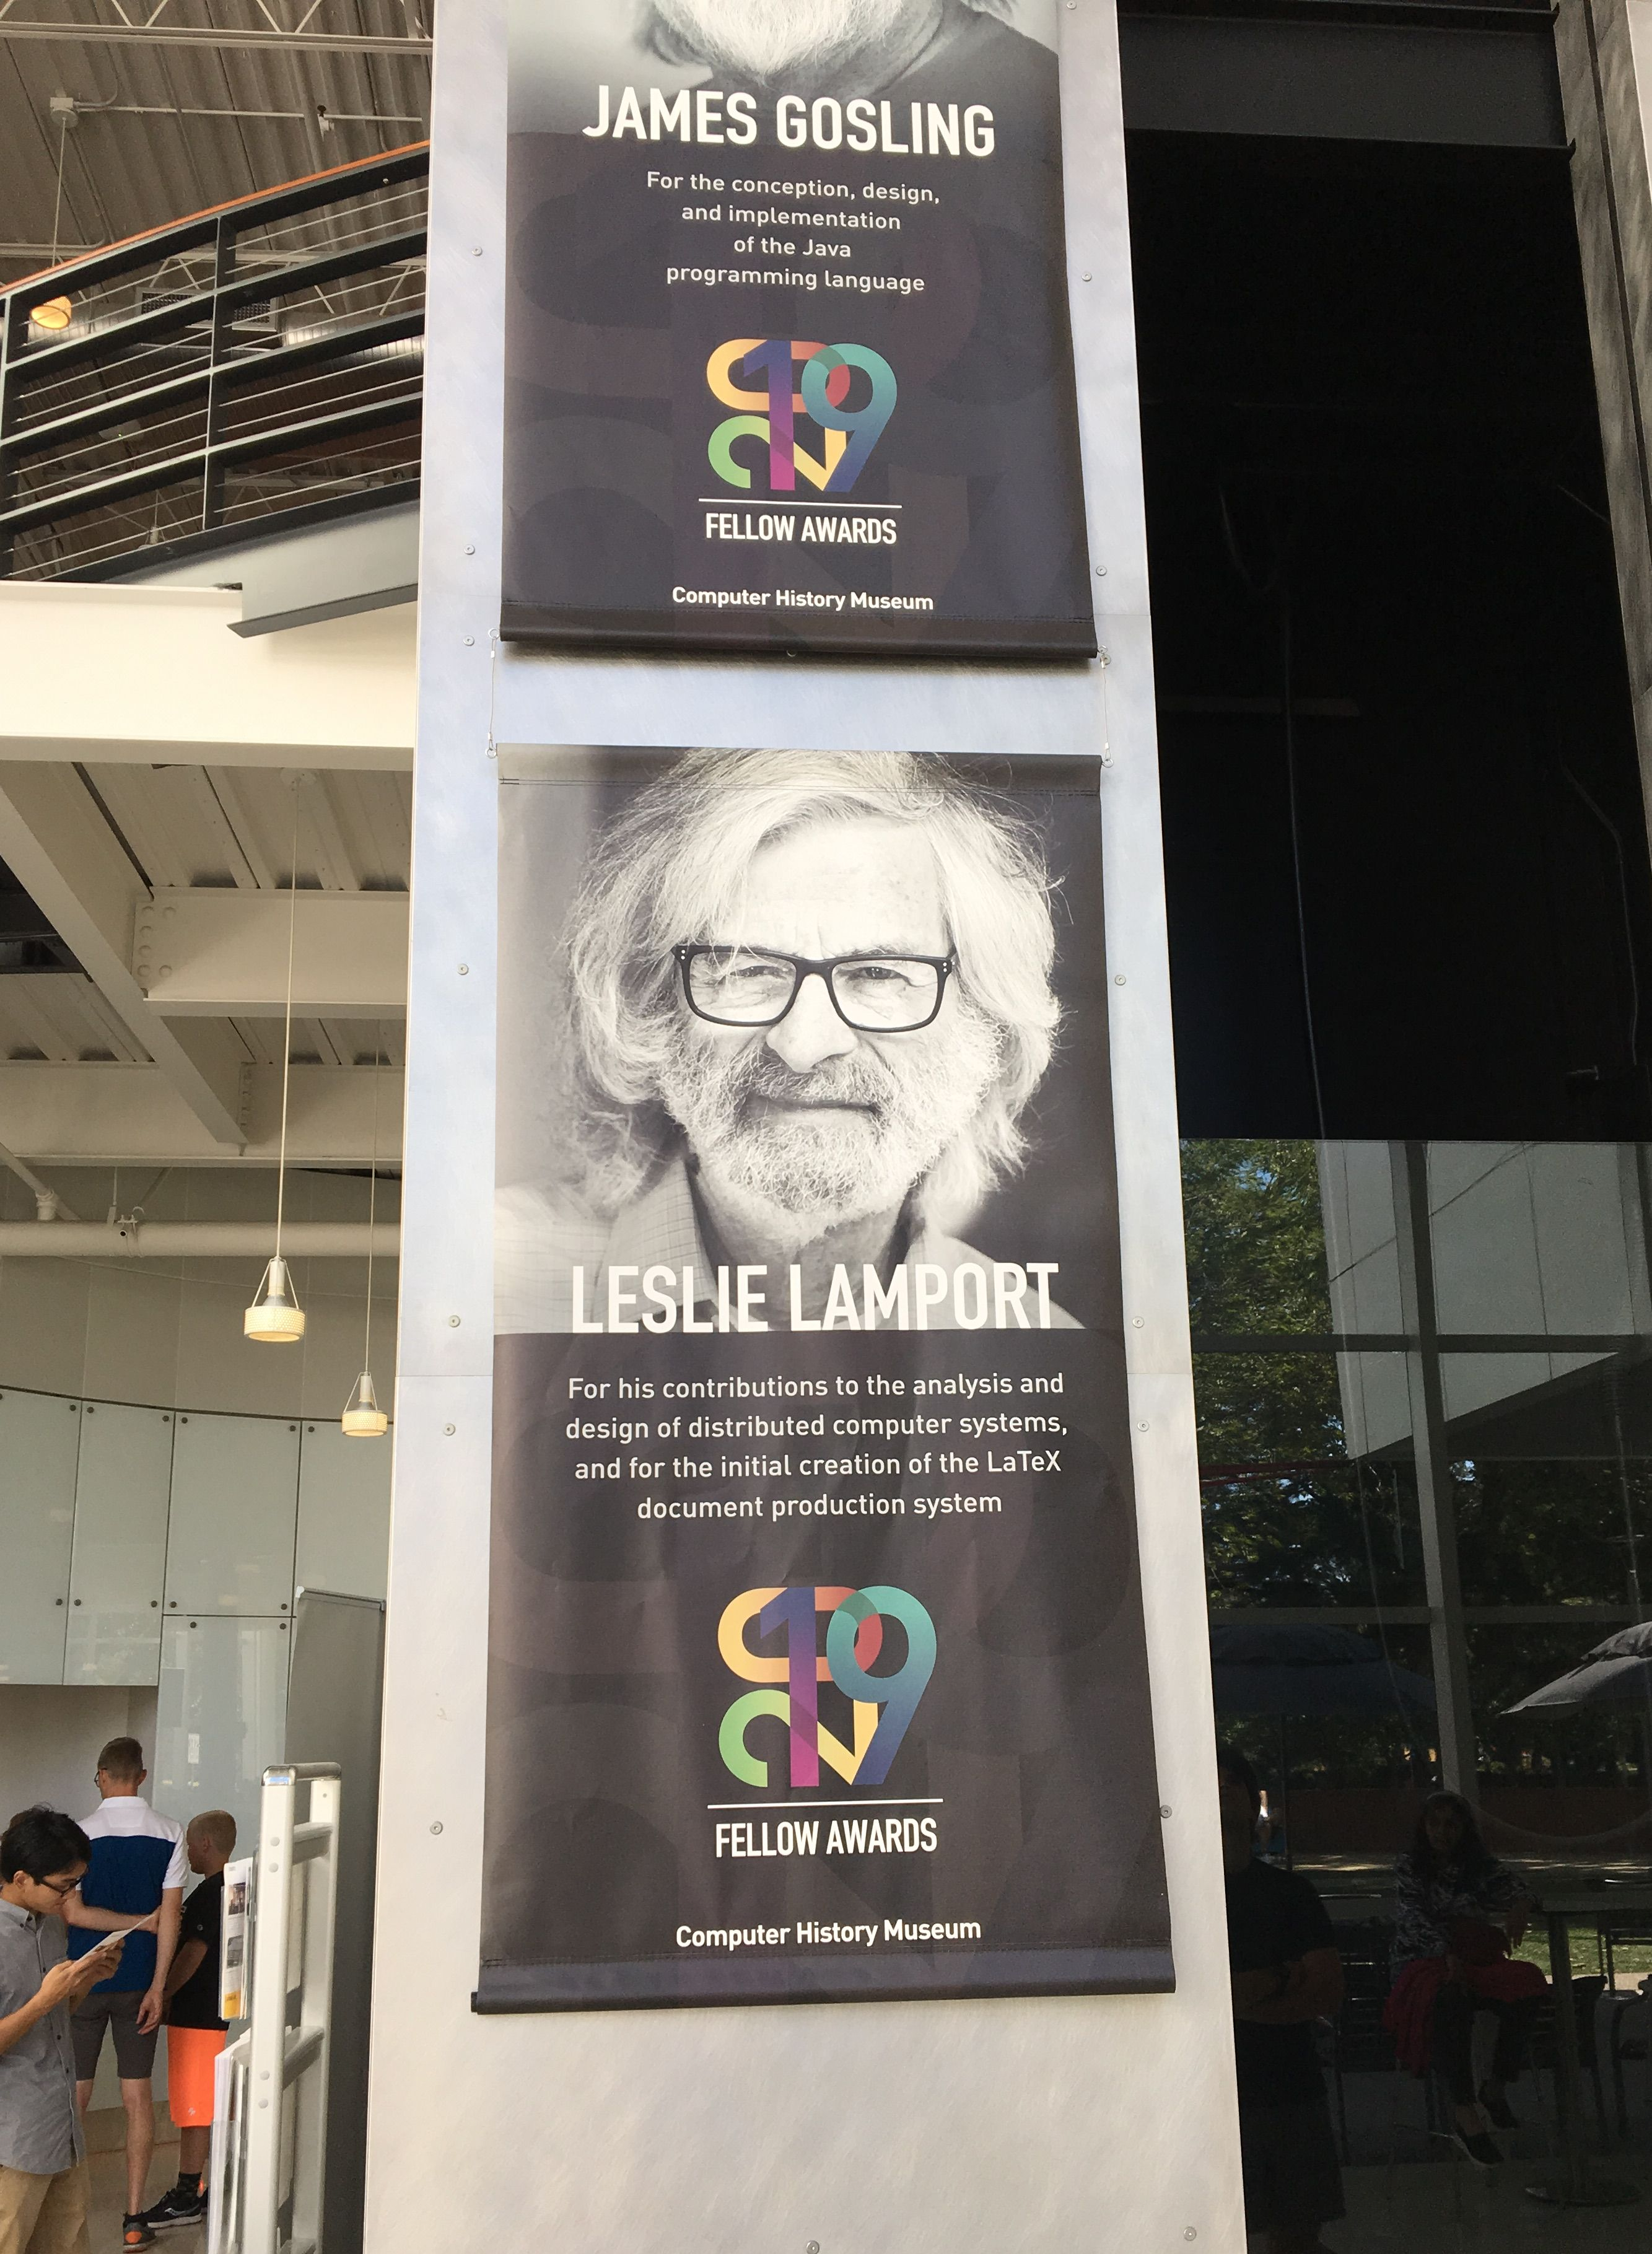
\includegraphics[height=0.8\textheight]{CHM}
\caption{Banner von Leslie Lamport im Computer History Museum, mit Erwähnung von \LaTeX}
\end{center}
\end{figure}

Nach dem folgenden Vortrag von Didier Verna zum Thema \enquote{Quickref und TeXinfo} hielt ich dann meinen zweiten Vortrag, diesmal zum \enquote{exam} Paket, mit dem sich sehr gut Klausuren und Übungszettel setzen lassen. Die Folien und der TUGboat-Artikel dazu sind auf \url{www.uweziegenhagen.de} verfügbar.

Die beiden folgenden Vorträge, von Chris Rowley und Ross Moore, behandelten dann das Thema Barrierefreiheit im \LaTeX-Kernel und die Erzeugung barrierefreier Dokumente. Die beiden Vorträge sind auch als Video verfügbar, man findet sie unter \url{http://web.science.mq.edu.au/~ross/TaggedPDF/TUG2019-movies/index.html}

Diese beiden Vorträge bildeten dann auch den Abschluss der TUG~2019. Am darauffolgenden Tag war es dann auch Zeit für mich, wieder nach Deutschland zurückzukehren. Zusammenfassend kann man sagen, dass insbesonderere diese TUG-Tagung deutlich technischer war und näher am \TeX-Kern als die Dante-Tagungen. Es war schön zu sehen, dass selbst nach vierzig Jahren noch so intensiv am \TeX-Kern gerarbeitet wird.

\end{document}



